\subsection{Pressure Drop}

Before analyzing thermal results from the CFD-DEM coupling, the system was run at various particle Reynolds numbers and the overall pressure drop of the packed bed was measured with a varied constant inlet velocity. This value was compared against the well-known Kozeny-Carman and Ergun equations; however the Kozeny-Carman is known to fit better with experimental data at very small Reynolds numbers. In Fig.~\ref{fig:cfdem-pressure-drop} we see the CFD-DEM coupling model is providing bed-scale pressure drops that match very well with Kozeny-Carman over the Reynold’s numbers applicable to helium purge flow in fusion reactors. This is the sole validation effort performed on the CFD-DEM tool.

\begin{figure}
        \centering
        \begin{subfigure}[b]{0.7\textwidth}
                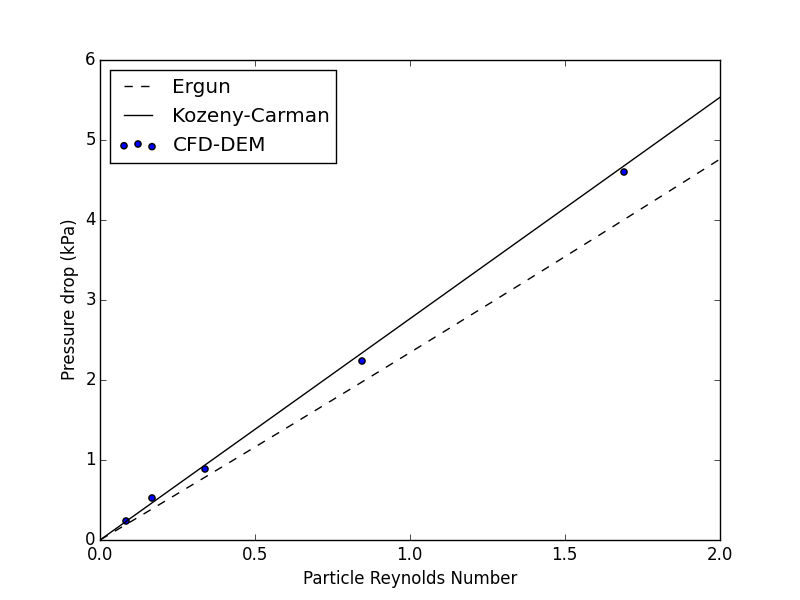
\includegraphics[width=\textwidth]{chapters/figures/pressureDrops-full.png}
                \caption{Well-packed bed}
                \label{fig:pressure-drop-full}
        \end{subfigure}%
        
          %add desired spacing between images, e. g. ~, \quad, \qquad, \hfill etc.
          %(or a blank line to force the subfigure onto a new line)
        \begin{subfigure}[b]{0.7\textwidth}
                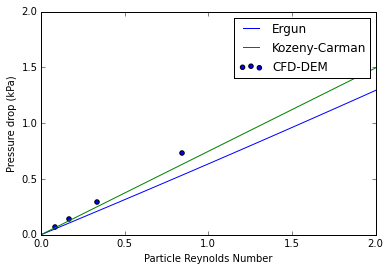
\includegraphics[width=\textwidth]{chapters/figures/pressureDrops-evap.png}
                \caption{Re-settled bed}
                \label{fig:pressure-drop-evap}
        \end{subfigure}
        \caption{Pressure drop calculations across packed beds, solved by CFD-DEM, fit well to the Kozeny-Carman empirical relation.}\label{fig:cfdem-pressure-drop}
\end{figure}